30. \begin{figure}[ht!]
\center{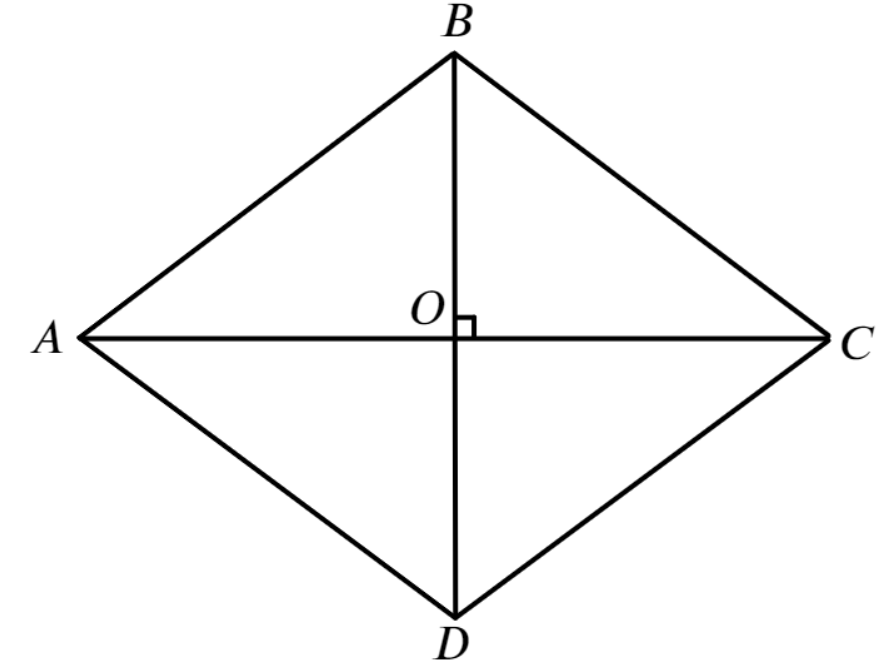
\includegraphics[scale=0.35]{g9-29.png}}
\end{figure}\\
В ромбе диагонали перпендикулярны и делятся точкой пересечения пополам. Если $BD=6$см, то по теореме Пифагора $AO=\sqrt{25-9}=4$см, значит вторая диагональ равна 8 см. Площадь ромба равна половине произведения диагоналей, значит $S=\cfrac{1}{2}\cdot6\cdot8=24\text{ см}^2.$
ewpage
oindent
